% !TeX root = ../main.tex

\section{1D Digital filters}
\begin{center}
    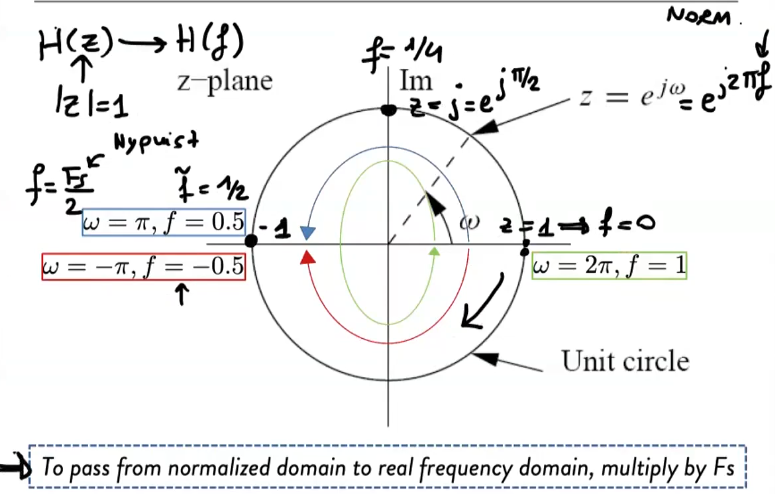
\includegraphics[width=1\textwidth]{images/zero_pole.png}
\end{center}
If asks for $Hz$ domain, multiply by $F_s$. Reminder, a filter:
\begin{LARGE}    
    $$
    H(z)=\frac{
        \sum_{k=0}^Nb_kz^{-k}
    }{\sum_{k=0}^Da_kz^{-k}}=
    z^{D-N}\frac{b_0}{a_0}\frac{
        \prod_{i=1}^N(z-z_i)
    }{\prod_{i=1}^N(z-p_i)}=
    \frac{b_0}{a_0}\frac{
        \prod_{i=1}^N(1-z_iz^{-1})
    }{\prod_{i=1}^N(1-p_iz^{-1})}
    $$
\end{LARGE}
\begin{itemize}
    \item The poles
    \begin{itemize}
        \item Are associated with the autoregressive part, they generate IIR filter $z\rightarrow p_i$, in the frequency the filter will increase $H(f)$
        \item The filter amplitude response enhances frequencies which are near the poles
        \item If poles are outside the unit circle and the filter is causal, the system is unstable
    \end{itemize}
    \item The zeros
    \begin{itemize}
        \item Are associated with the moving average of the filter, they generate FIR filters
        \item The filter amplitude response attenuates frequencies which are near the zero
        \item Zeros influence also the phase of the filter (they do not influence stability)
        \begin{itemize}
            \item Minimum phase zeros if $z<1$, inside unit circle
            \item Maximum phase zeros if $z\geq 1$, outside unit circle
        \end{itemize}
    \end{itemize}
\end{itemize}

\subsection{Filter design: remarkable LTI filters}
\begin{itemize}
    \item Place poles close tot he unit circle in frequencies that must be emphasized
    \item Place zeros according to the desired phase response, the closer are to the unit circle the higher frequency attenuation
\end{itemize}

\subsubsection{Notch}
I want to delete a specific frequency:
\begin{enumerate}
    \item Put two complex zeros on the unit circle
    \item Put two poles with absolute value less than 1, close to unit circle
\end{enumerate}
\begin{center}
    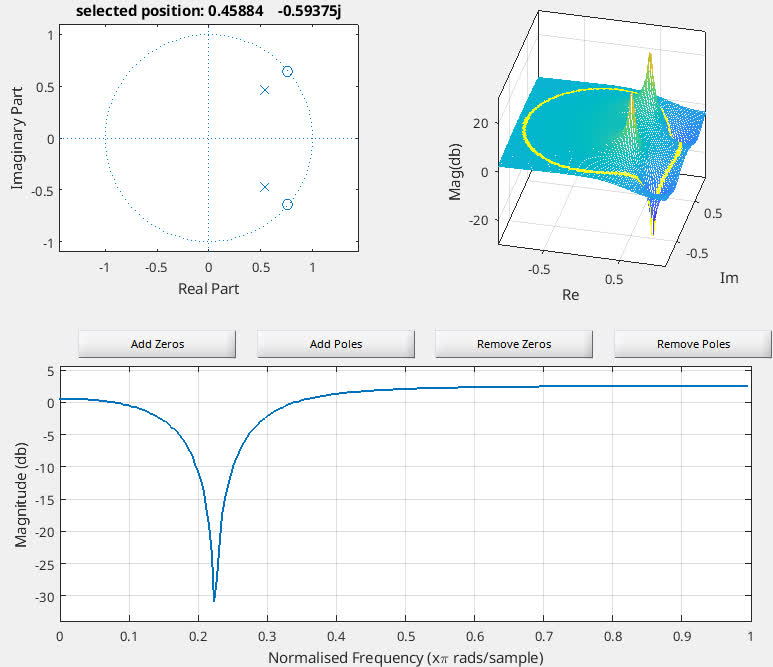
\includegraphics[width=1\textwidth]{images/notch.png}
\end{center}

\subsubsection{Magnitude square function}
The magnitude response of a LTI system is:
$$
M(f)=|H(f)|^2=H(f)\cdot H^*(f)=H(z)\cdot H^*(z^{-1})\big|_{|z|=1}
$$
Given a generic rational transfer function
$$
H(z)=\frac{b_0}{a_0}\frac{
    \prod_{i=1}^N(1-z_iz^{-1})
}{\prod_{i=1}^N(1-p_iz^{-1})}
$$
$$
\Downarrow
$$
$$
M(z)=H(z)H^*(z^{-1})=\frac{|b_0|^2}{|a_0|^2}
\frac{
    \prod_{i=1}^N(1-z_iz^{-1})(1-z_i^*z)
}{\prod_{i=1}^D(1-p_iz^{-1})(1-p_i^*z)}
$$
Where $H^*(z^{-1})$ means $H(z)$ with complex conjugates evaluated in $z^{-1}$, star in the coefficients
\begin{itemize}
    \item For each zero $z_i$ of $H(z)$ there is another zero at $\frac{1}{z_i^*}$
    $$
    \frac{1}{z_i^*}=\frac{1}{\rho_ie^{-j\theta_i}}=\frac{1}{\rho_i}e^{j\theta_i}
    $$
    The angle/phase is the same, only distance from origin changes
    \item For each pole $p_i$ of $H(z)$ there is another pole at $\frac{1}{p_i^*}$
    \item $M(z)$ presents poles and zeros in conjugate reciprocal pairs
\end{itemize}
\begin{center}
    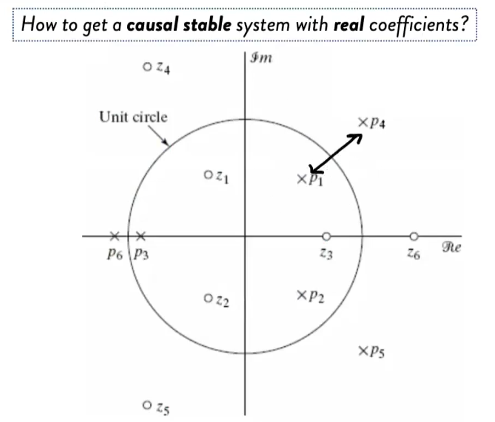
\includegraphics[width=0.6\textwidth]{images/magnitued_square.png}
\end{center}
Given a magnitude response requirement $M(z)$ for $H(z)$, given stability and causality requirements for $H(z)$:
\begin{itemize}
    \item The poles of $H(z)$ are those of $M(z)$ inside the unit circle anda re uniquely identified (for stability constraints)
    \item The zeros of $H(z)$ are not uniquely identified (as zeros influence only the phase and we have no constraints on phase), so the zeros can be both inside and outside the unit circle
    \item Given a causal FIR filter $H(z)$ of order $N$, it has the same magnitude  response $M(z)$ of the causal FIR filter:
    $$G(z)=z^{-N}H^*(z^{-1})$$
    Minimum to maximum phase filter and viceversa
\end{itemize}
From the previous example, in order to have causal and stable system we select the following zeros and poles:
\begin{center}
    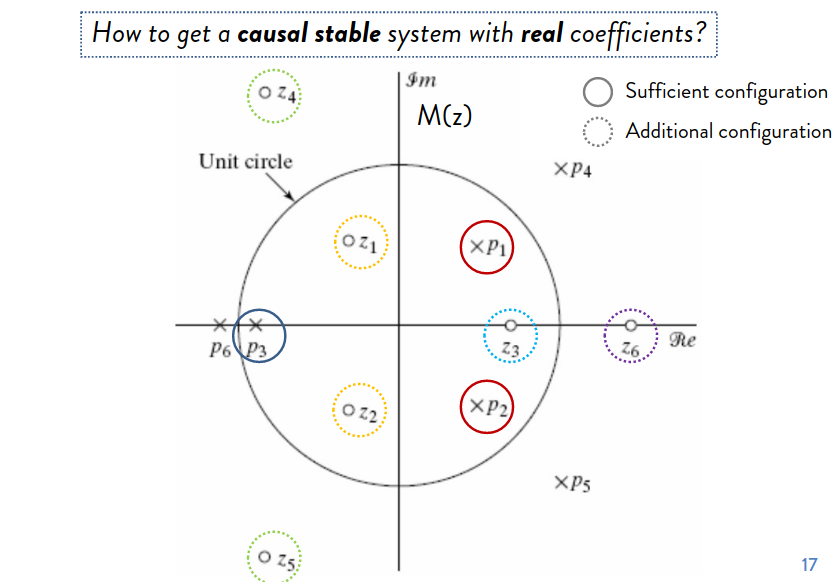
\includegraphics[width=0.6\textwidth]{images/magnitued_square2.png}
\end{center}

\subsubsection{Allpass filters}
Flat behavior in the frequency, which means constant gain and any phase:
$$
|H_{ap}(f)|=|H_{ap}(z)|\big|_{|z|=1}=1\qquad\forall f
$$
Given the previous considerations, a generic causal allpass filter is:
$$
H_{ap}(z)=z^{-K}e^{j\phi}\frac{A(z)}{\tilde{A}(z)}
$$
Where
$$
\begin{cases}
    A(z)=1+a_1z^{-1}+a_2z^{-2}+\cdots+a_Nz^{-N}\\
    \tilde{A}(z)=z^{-N}A^*(z^{-1})=a^*_N+a_{N-1}^*z^{-1}+\cdots+a_2^*z^{2-N}+a_1^*z^{1-N}+z^{-N}
\end{cases}
$$
The denominator is the G version of the numerator, so their magnitudes cancel out.
$$
H_{ap}(z)=z^{-N}e^{j\theta}
\frac{
    1+a_1z^{-1}+a_2z^{-2}+\cdots+a_Nz^{-N}
}{
    a^*_N+a_{N-1}^*z^{-1}+\cdots+a_2^*z^{2-N}+a_1^*z^{1-N}+z^{-N}
}
$$
A general form to represent an allpass real valued impulse response is:
\begin{center}
    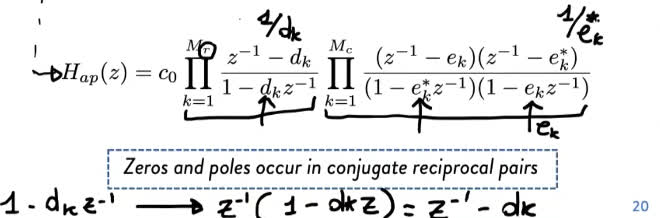
\includegraphics[width=0.6\textwidth]{images/allpass.png}
\end{center}
We introduced a coefficient $c_0$ in order to guarantee magnitude of 1. Basically
$$
H(z)=\left|c_0\frac{B_{ap}(z)}{A_{ap}(z)}\right|_{|z|=1}=1
$$
We pass to the frequency domain. As that fraction is flat in the frequency domain, we choose frequency $f=0,z=1$:
$$
|c_0|\frac{|B_{ap}(z=1)|}{|A_{ap}(z=1)|}=1
$$
$$
\Rightarrow c_0 = \pm\frac{|A_{ap}(z=1)|}{|B_{ap}(z=1)|}
$$
So to find $c_0$ just sum  all the coefficients and then compute the division.

\textbf{Zeros and poles are in conjugate reciprocal pairs}.
Properties:
\begin{itemize}
    \item Cascade of two allpass filters is again an allpass filter
    \item Each pole of an allpass system is associated with a conjugate reciprocal zero
    \item The magnitude of many cascaded allpass filters is always the same
\end{itemize}

\subsubsection{Minimum phase filters}
\begin{itemize}
    \item Minimum phase filters are such that both $H(z)$ and $\frac{1}{H(z)}$ are stable and causal
    \item The poles must be inside the unit circle
    \item The zeros must be inside the unit circle
    \item Given a square magnitude response $M(z)$, there is a unique system whose zeros and poles are inside the unit circle and it is called minimum phase system
\end{itemize}
\begin{center}
    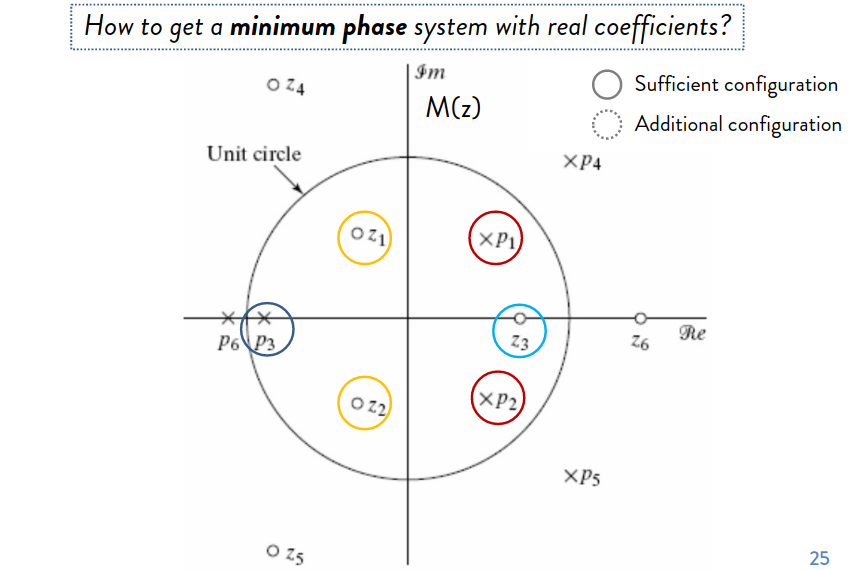
\includegraphics[width=0.8\textwidth]{images/minphase.png}
\end{center}
Properties of allpass: \textbf{Any rational causal stable system can be decomposed into the multiplication of a minimum phase system and an allpass system}
$$
H(z)=H_{min}(z)H_{ap}(z)
$$
Causal and stable, so all poles are inside the unit circle!\\
$H_{min}(z)$ contains:
\begin{itemize}
    \item The poles and the zeros of $H(z)$ that lie inside the unit circle
    \item Zeros that are conjugate reciprocals of the zeros $H(z)$ lying outside the unit circle
\end{itemize}
$H_{ap}(z)$ contains:
\begin{itemize}
    \item All the zeros of $H(z)$ that lie outside the unit circle
    \item Poles that are conjugate reciprocals of the zeros of $H(z)$ lying outside the unit circle
\end{itemize}

\subsection{Digital filters' design}
\begin{enumerate}
    \item Specify always the characteristics of the filter in frequency domain, not in time domain (e.g. lowpass, highpass, bandpass...)
    \item Approximate these properties using a discrete-time system, find the filter coefficients
    \item Realize the system using finite precision arithmetic
\end{enumerate}

\subsubsection{Ideal filters}
\begin{center}
    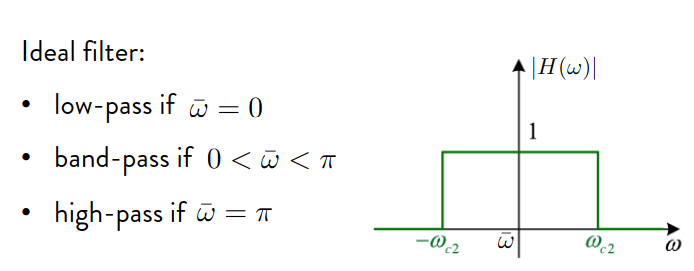
\includegraphics[width=0.8\textwidth]{images/idealfilter.png}
\end{center}
Outside the rectangle is called \textbf{stopband}. The impulse response of this filter is $\approx$ the sinc function. It is \textbf{non-causal (sinc has on the left non-causal part)} with an \textbf{infinite delay}, \textbf{real systems can only approximate}.

\subsubsection{Real filters}
\begin{center}
    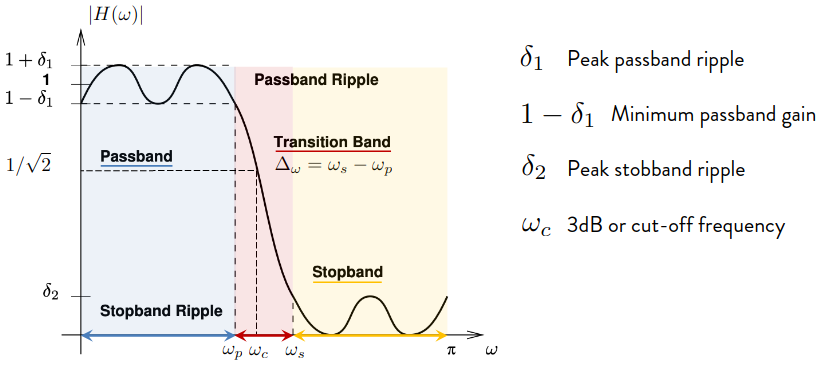
\includegraphics[width=1\textwidth]{images/realfilter.png}
\end{center}
Oscillations both in passband and in stopband. Cutoff frequency is the frequency in which I pass from the passband to the stopband.

As I don't want ripples and we want transition band to 0:
\begin{itemize}
    \item Peak ripple $\rightarrow$ 0
    \item Transition band $\rightarrow$ 0
\end{itemize}
We consider FIR and IIR cases:
\begin{center}
    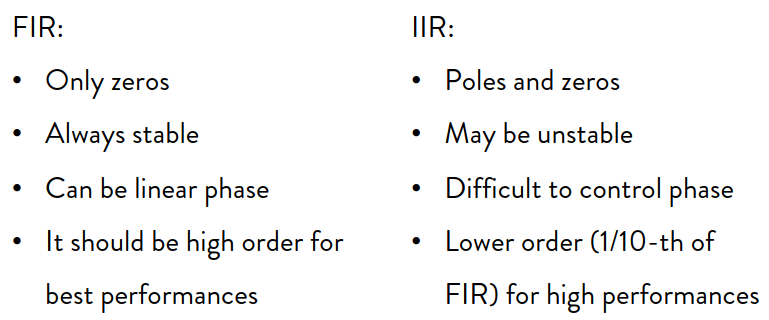
\includegraphics[width=1\textwidth]{images/IIRvsFIR.png}
\end{center}
Allpass must be FIR.

\subsubsection{FIR filter design: windowing method}
I want a rectangle in the frequency, but in the time I have a sinc: obtain a FIR filter by truncating an infinite duration impulse response
\begin{itemize}
    \item Given the ideal $h_i(n)$, build $h(n)=h_i(n)w(n)$
    \item $w(n)$ is a finite duration window, in frequency domain it becomes convolution
    \item $H(f)$ is a blurred version of the ideal filter $H_i(f)$
\end{itemize}
\textbf{Windowing means multiplying in the time, so in the frequency we have convolution}.

How to choose the window? Tradeoff
\begin{itemize}
    \item As short as possible (in time) to minimize the cost of the FIR filter
    \item As narrow as possible in frequency to approach the ideal filter (a narrow in the time means very large in the frequency domain)
\end{itemize}
I want a short signal in the time, so an impulse, $W(f)$ should look like a $\delta(f)$, without considering the filter cost
\begin{itemize}
    \item Its energy must be concentrated around $f=0$
    \item $W(f)$ should decay fast as frequency increases
\end{itemize}
\begin{center}
    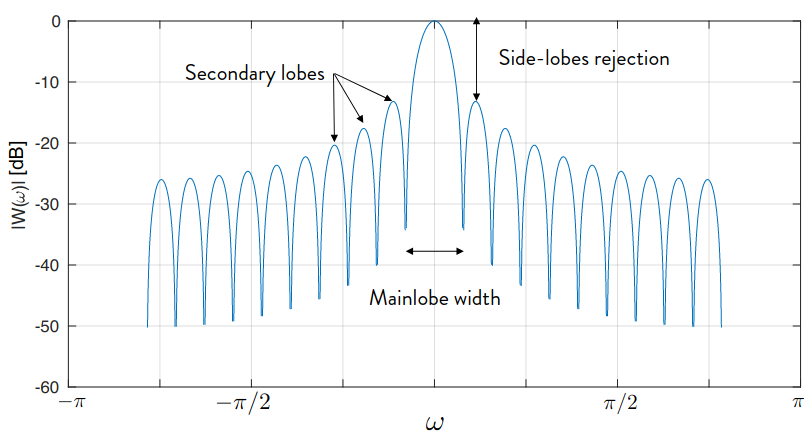
\includegraphics[width=1\textwidth]{images/lobe.png}
\end{center}
We want a big ration of $\frac{width(MainLobe)}{width(SecondaryLobes)}$. Every window is characterized by:
\begin{itemize}
    \item Main-lobe width: it decreases as the window length increases
    \item Side-lobes rejection: ratio between the main-lobe peak and 1° secondary lobe peak [dB], if I want it high for example the blackman window is quite good
    \item Side-lobes roll off: asymptotic decay of the side-lobe peaks vs frequency octave [dB/octave] or frequency decade [dB/decade
\end{itemize}
\textbf{In matlab set cutoff = double of desired one, if I want cutoff of 0.5 I will put in matlab 1}.

\subsection{Aspects to remember}
\begin{itemize}
    \item \textbf{Phase is always correlated with a delay in the time}
    \item \textbf{Real filters always introduce a delay, a phase term}
    \item \textbf{FIR are always stable}, the numerator has greater grade than denominator
    \item \textbf{Allpass MUST be FIR}
    \item \textbf{Only poles in the origin means FIR}
    \item \textbf{Denominator = 1 means FIR}
    \item \textbf{Maximum phase will result in jumps in the phase plot}
    \item \textbf{Minimum phase has the greatest part of energy of the filter concentrated in the first part of the temporal samples}, which means I am introducing very small delay
    \item \textbf{DFT of sinusoid will have peak in the freq/normalized freq depending on representation of frequency domain ($f_0\,\,[Hz]|\tilde{f_0}$) and another one symmetric w.r.t. Nyquist frequency}
\end{itemize}

